\documentclass[a4paper,11pt,dvipdfmx]{ujarticle}
% パッケージ
\usepackage{graphicx}
\usepackage{url}
% レイアウト指定を記述したファイルの読み込み
\input{layout}

\title{日本におけるデジタル化の状況}
\author{G584782025 藤戸 慎汰}
\begin{document}
\maketitle 

\section{デジタル競争力ランキング}
国際経営開発研究所(IMD)の調査\cite{IMD}によると、
日本のデジタル競争力ランキングは図\ref{fig:graph}を示すように、
調査対象の64カ国中、総合で28位、準備分野で27位となっている。
\begin{figure}[htbp]
    \centering
    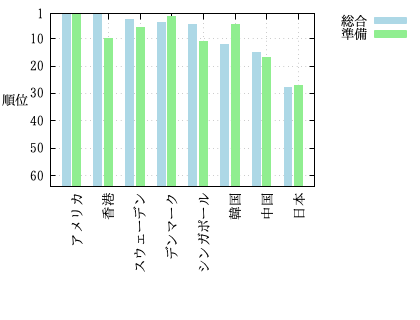
\includegraphics{graph.png}
    \caption{デジタル競争力ランキング(64カ国中)}\label{fig:graph}
\end{figure}

\newpage
\section{ブロードバンドの整備状況}
% 本文(2)
OECDによるブロードバンド回線の普及に関する調査\cite{oecd}によると、表\ref{tbl:table}に示すように、日本における 100人あたりのモバイルブロードバンドの加入者数は190.5で、第1位になっている。2位はエストニア
で、3位米国と続く。
\begin{table}[htbp]
    \centering
    \caption{モバイルブロードバンドの加入者数(100人あたり)}\label{tbl:table}
    \begin{tabular}{|c|c|c|}
        \hline
        順位 & 国名 & 加入者数 \\
        \hline
        1位 & 日本 & 190.5 \\
        \hline
        2位 & エストニア & 179.9 \\
        \hline
        3位 & 米国 & 169.0 \\
        \hline
        4位 & フィンランド & 157.0 \\
        \hline
        5位 & デンマーク & 141.7 \\
        \hline
        6位 & ラトビア & 141.6 \\
        \hline
        7位 & イスラエル & 139.9 \\
        \hline
        8位 & オランダ & 133.7 \\
        \hline
        9位 & ポーランド & 131.3 \\
        \hline
        10位 & スウェーデン & 127.2 \\
        \hline
    \end{tabular}
\end{table}

\section{考察}
上記の内容から次のことが考えられる。
\begin{itemize}
    \item 日本が今後の企業が海外に対抗するためには企業がデジタル技術を使った効率化などの技術革新を行う必要性が考えられる。
    \item モバイルブロードバンドを提供する企業が海外進出を進め、さまざまな国で5G通信が行えるようになることが、各国の普及率増加につながると考えられる。
\end{itemize}

\bibliographystyle{junsrt}
\bibliography{exercise.bib}

\end{document}